% UQ Gemini theme
% See: https://github.com/alfurka/gemini-uq
% Forked from
% https://rev.cs.uchicago.edu/k4rtik/gemini-uccs
% which is forked from
% https://github.com/anishathalye/gemini


\documentclass[final]{beamer}

% ====================
% Packages
% ====================

\usepackage[T1]{fontenc}
\usepackage{lmodern}
\usepackage[size=custom,width=91.44,height=121.92,scale=1.42]{beamerposter}
\usetheme{gemini}
\usecolortheme{uchicago}
\usepackage{graphicx}
\usepackage{booktabs}
\usepackage{tikz}
\usepackage{pgfplots}
\usepackage{cite}
%\usepackage[UTF8]{ctex}
\pgfplotsset{compat=1.17}

% ====================
% Lengths
% ====================

% If you have N columns, choose \sepwidth and \colwidth such that
% (N+1)*\sepwidth + N*\colwidth = \paperwidth
\newlength{\sepwidth}
\newlength{\colwidth}
\setlength{\sepwidth}{0.025\paperwidth}
\setlength{\colwidth}{0.3\paperwidth}

\newcommand{\separatorcolumn}{\begin{column}{\sepwidth}\end{column}}

% ====================
% Title
% ====================

\title{SINGLE-CHANNEL TARGET SPEAKER SEPARATION USING JOINT TRAINING WITH TARGET SPEAKER'S PITCH INFORMATION}

\author{Jincheng He \inst{1}, Yuanyuan Bao\inst{1}, Na Xu\inst{2}, Hongfeng Li \inst{2}, Shicong Li\inst{2}, Linzhang Wang\inst{2}, Fei Xiang\inst{2}, Ming Li\inst{1}}

\institute[shortinst]{\inst{1} Data Science Research Center, Duke Kunshan University, Kunshan, China \samelineand \inst{2} Xiaomi, Beijing, China \\ ming.li369@duke.edu}

% ====================
% Footer (optional)
% ====================

%\footercontent{
%    \href{https://www.example.com}{https://www.example.com} \hfill
%    ABC Conference 2025, New York --- XYZ-1234 \hfill
%    \href{mailto:a.kalay@example.com}{a.k@example.com}}
% (can be left out to remove footer)

% ====================
% Logo (optional)
% ====================

% use this to include logos on the left and/or right side of the header:
% \logoright{\includegraphics[height=7cm]{logo1.pdf}}
% \logoleft{\includegraphics[height=7cm]{logo2.pdf}}

% ====================
% Body
% ====================

\begin{document}
    \addtobeamertemplate{headline}{}
%    {
%        \begin{tikzpicture}[remember picture,overlay]
%            \node [anchor=north west, inner sep=3cm] at ([xshift=0.0cm,yshift=1.0cm]current page.north west)
%                {
\includegraphics[height=5.0cm]{logos/Logo-Left.png}}; % also try shield-white.eps
%            \node [anchor=north east, inner sep=3cm] at ([xshift=0.0cm,yshift=2.5cm]current page.north east)
%                {
\includegraphics[height=8.0cm]{logos/Logo-Right.png}};
%        \end{tikzpicture}
%    }

    \begin{frame}[t]
        \begin{columns}[t]
            \separatorcolumn

            \begin{column}{\colwidth}

                \begin{block}{Abstract}
                    Despite the great progress achieved in the target speaker separation (TSS) task, we are still trying to find other robust ways for performance improvement which are independent of the model architecture and the training loss. Pitch extraction plays an important role in many applications such as speech enhancement and speech separation. It is also a challenging task when there are multiple speakers in the same utterance. In this paper, we explore if the target speaker pitch extraction is possible and how the extracted target pitch could help to improve the TSS performance. A target pitch extraction model is built and incorporated into different TSS models using two different strategies, namely concatenation and joint training. The experimental results on the LibriSpeech dataset show that both training strategies could bring significant improvements to the TSS task, even the precision of the target pitch extraction module is not high enough.

                    \begin{keywords}
                        target speaker separation, target pitch extraction, joint learning
                    \end{keywords}
                \end{block}

                \begin{block}{Introduction}
                    Target speaker separation (TSS) has attracted much attention in recent years~\cite{speakerBeam, compact_speakerbeam, voicefilter, li20p_interspeech, time_domain_speaker_ex_net, spex, spex+, speakerfilter, speakerfilter_pro}.
                    It is the task which only extracts the speech of the target speaker in the environment with multiple people speaking simultaneously.
                    The general deep neural network based TSS framework could be summarized as an Encoder (including the speech and speaker encoder)-Separator-Decorder architecture, shown as Figure~\ref{fig:enc_sep_doc_arc}.

                    The related works, such as VoiceFilter~\cite{voicefilter}, Atss-Net~\cite{li20p_interspeech}, spex++~\cite{time_domain_speaker_ex_net, spex, spex+}, made efforts in different parts of the aforementioned architecture. The Atss-Net introduced attention mechanisms in the separator. The spex++ adopted the time-domain method and made lots of changes in the speech and speaker encoder. All of them contribute a lot to the development of TSS task.

                    Despite the great progress made, we are motivated to explore useful and robust training strategies that could be applied to different model architectures. For instance, use new feature as one of the inputs of separator.

                    Pitch, or fundamental frequency, is an important characteristic of speech and music signals.
                    The task of pitch extraction, or pitch tracking has a long history. There are multiple signal processing based methods to extract pitches. A time domain signal processing method is proposed in~\cite{yin} to estimate the foundamental frequency.
                    A frequency-domain signal processing method is proposed in~\cite{swipe}.

                    Before the usage of DNN methods for extracting pitches, there are some traditional signal processing methods, and although they have the advantage that the algorithms are easy to understand and do not
                \end{block}

            \end{column}

            \separatorcolumn

            \begin{column}{\colwidth}
                \begin{block}{}
                    require training data, they have limitations in terms of accuracy especially in complex environments. Hence, many machine learning based algorithms were developed.
                    A supervised machine learning based algorithm based in the time domain is proposed in~\cite{crepe}.
                    A self-supervised machine learning based algorithm in the frequency domain is proposed in~\cite{spice}.
                    Using pitch information to help speech separation task also attracts a lot of attention in recent years.
                    A pitch extraction module is concatenated with the separation module together to perform the separation task in~\cite{pitch_aware}.
                    A serial model is built and design the final loss as a weighted loss with the speech separation loss and pitch loss in~\cite{serial}. However the serial model in~\cite{serial} needs to go through the target speaker extraction first and then perform the pitch tracking after the extraction.

                    \begin{figure}[!t]
                        \centering
                        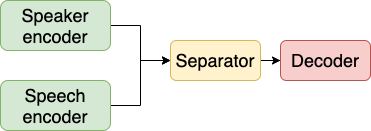
\includegraphics[width=0.58\linewidth]{img/encoder_sep_decoder}
                        \caption{The Encoder-Separator-Decoder architecture}
                        \label{fig:enc_sep_doc_arc}
                    \end{figure}

                    In our paper, we propose a target speaker pitch extraction module which can directly estimate the target speaker's pitch from a mixture of utterances from multiple speakers.
                    Then we explore the strategies on how to contribute this target speaker's pitch information to the target speaker separation task.
                    We propose a small scale Multi-Block RNNoise (MBRNN) model as our baseline speech separation system.
                    Then we propose two training strategies, namely concatenation training and joint training.
                    We further implement these two strategies on multiple models with different scales and the experiment results show that the joint training of the target pitch extraction model and the target speaker separation model is useful to improve the separation performance.
                    The proposed strategies could make positive impact on the TSS task even though the precision of the target pitch extraction is not high enough.
                    The performance of concatenation with ground-truth pitch information show great potential in utilizing the target speaker's pitch information for the TSS task.
                \end{block}

                \begin{block}{Acknowledgment}
                    This research is funded in part by the National Natural Science Foundation of China (62171207), the Fundamental Research Funds for the Central Universities (2042021kf0039), Key Research and Development Program of Jiangsu Province (BE2019054), Science and Technology Program of Guangzhou City (201903010040,202007030011), Xiaomi, Office of Undergraduate Studies and the DKU Summer Research Scholars Program.
                \end{block}

            \end{column}
            \separatorcolumn
            \begin{column}{\colwidth}
                \begin{block}{References}

%                    \nocite{*}
                    \footnotesize{\bibliographystyle{IEEEbib}\bibliography{ref}}

                \end{block}
            \end{column}

            \separatorcolumn
        \end{columns}
    \end{frame}

\end{document}
